\documentclass[11pt]{sdm}

\usepackage{graphicx}
\graphicspath{{../img/}}

\usepackage{subcaption}
\usepackage{cleveref}

\pagestyle{plain}

\usepackage{hyperref}
\usepackage{url} \urlstyle{sf}
\newcommand{\email}[1]{\href{mailto:#1}{#1}}

\usepackage{xspace}

\usepackage[dvipsnames]{xcolor}
\newcommand{\addref}[1]{\colorbox{TealBlue!100}{\textcolor{white}{\textbf{$[$\ifx&#1&\ \else#1\fi$]$}}}}
\newcommand{\todo}[1]{\colorbox{Red!75}{\textcolor{white}{\textbf{TODO\ifx&#1&\else: #1\fi}}}}
\newcommand{\done}{\colorbox{YellowGreen!100}{\textcolor{white}{\textbf{DONE}}}}
\newcommand{\review}{\colorbox{YellowOrange!100}{\textcolor{white}{\textbf{REVIEW}}}}

\newcommand{\dspot}{DSpot\xspace}
\newcommand{\pitest}{Pitest\xspace}

\usepackage{listings}
\lstset{%
%  backgroundcolor=\color{white},   % choose the background color; you must add \usepackage{color} or \usepackage{xcolor}
  basicstyle=\small,        % the size of the fonts that are used for the code
  captionpos=b,                    % sets the caption-position to bottom
  commentstyle=\color{cyan},    % comment style
  escapeinside={(*@}{@*)},          % if you want to add LaTeX within your code
  keywordstyle=\color{blue},       % keyword style
  stringstyle=\color{red},       % keyword style
  numberstyle=\tiny\color{black}, % the style that is used for the line-numbers
  stepnumber=1,                    % the step between two line-numbers. If it's 1, each line will be numbered
  title=\lstname,                   % show the filename of files included with \lstinputlisting; also try caption instead of title
  language=Java,
  breakatwhitespace=false,         % sets if automatic breaks should only happen at whitespace
  breaklines=true,                 % sets automatic line breaking
  extendedchars=true,              % lets you use non-ASCII characters; for 8-bits encodings only, does not work with UTF-8
  %frame=single,                    % adds a frame around the code
  showspaces=false,                % show spaces everywhere adding particular underscores; it overrides 'showstringspaces'
  showstringspaces=false,          % underline spaces within strings only
  showtabs=false,                  % show tabs within strings adding particular underscores
  tabsize=2                       % sets default tabsize to 2 spaces
}

\title{Search-Based Test Amplification}

\author{Simon \textsc{Bihel}}
\supervisorOne{Benoit \textsc{Baudry}}
\supervisorTwo{}
\team{KTH Royal Institute of Technology}
\school{ens-Rennes}

\domain{Domain: Software Engineering - Artificial Intelligence}

\abstract{%
With the poor use of formal specifications for software development, programmers ensure the well-behavior of software with hand-written tests.%
Meta-heuristic optimizing techniques are used to automate the process of testing (e.g.\ generating test data).%
%
With practices such as test-driven development, software projects come with strong test suites.%
Knowledge of the expected properties of the program can be extracted from the large number of test cases.%
This knowledge can be used in turn to enhance the test suite to improve certain software metrics.%
%
Different goals can be pursued to reduce the likelihood of bugs, to help during debugging, etc.%
The amplification can be achieved by generating variants of existing tests, modifying the tests execution, etc.%
}

\date{February 2018}

% Ought to be 10 to 15 pages long

\begin{document}
\maketitle

\section*{Introduction}
\label{intro}

With the poor use of formal specifications for software development, programmers ensure the well-behavior of software with hand-written tests.
Meta-heuristic optimizing techniques are used to automate the process of testing (e.g.\ generating test data).
% target function is a software metric

With practices such as test-driven development, software projects come with strong test suites.
Knowledge of the expected properties of the program can be extracted from the large number of test cases.
This knowledge can be used in turn to enhance the test suite to improve certain software metrics.

Different goals can be pursued to reduce the likelihood of bugs, to help during debugging, etc.
The amplification can be achieved by generating variants of existing tests, modifying the tests execution, etc.
\todo{badly written}

After explaining the basics of Search-Based Software Testing in Section~\ref{sbse} we will present how it can be used to amplify test suites in Section~\ref{tsa}.
In Section~\ref{planned} we detail the different paths the internship could explore.


\section{Search-Based Software Engineering}
\label{sbse}

In this section we present the reasons for the emergence of Search-Based Software Engineering (SBSE)~\cite{harman2001search,mcminn2011search} and give examples of applications.

\subsection{Motivations}
\label{motiv}
\todo{}

Software projects are continuously getting more complex.
They often rely on informal specifications that change during the evolution of the project.
Because of the scale and weak structure, formal methods cannot be used in many cases.

In order to tackle problems such as optimization or testing, we need insightful approximating methods.

Over time software engineers have developed many metrics to evaluate a piece of software and get feedback on its quality.

\subsection{Search-Based Optimization Algorithms}
\label{example_algo}

To reach a software engineering goal for these complex systems we use \textit{soft-computing} (or \textit{computational intelligence}) to find inexact or sub-optimal solutions in a reasonable time.
In~\ref{basic_algo} we present some algorithms to give an idea of the capabilities of these techniques.
In~\ref{fitness_func} we show how we can pursue engineering goals with these optimization processes.

\subsubsection{Basic algorithms}
\label{basic_algo}

\begin{figure}
  \centering
  \begin{subfigure}[b]{0.3\textwidth}
    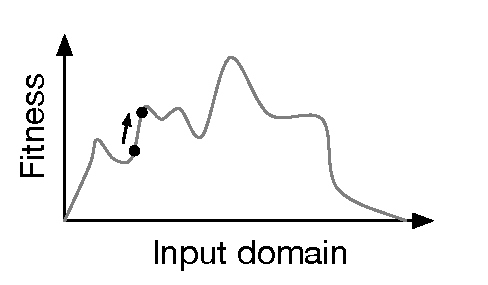
\includegraphics[width=\textwidth]{hillclimbing}
\caption{Hill Climbing}
\label{fig:hill_climbing}
  \end{subfigure}
  ~
  \begin{subfigure}[b]{0.3\textwidth}
    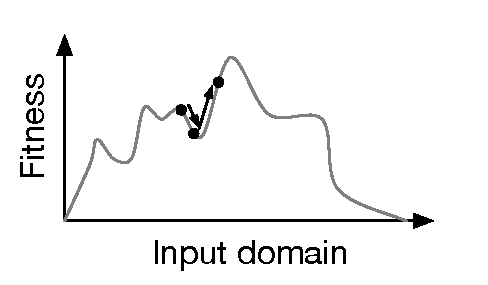
\includegraphics[width=\textwidth]{simulated_annealing}
\caption{Simulated Annealing}
\label{fig:simulated_annealing}
  \end{subfigure}
  ~
  \begin{subfigure}[b]{0.3\textwidth}
    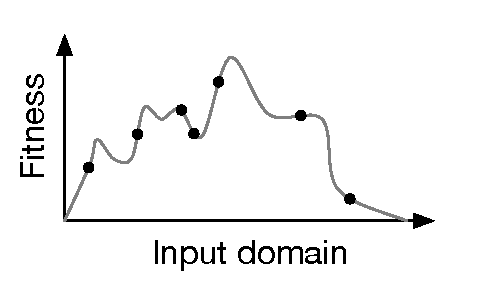
\includegraphics[width=\textwidth]{genetic_algo}
\caption{Genetic Algorithm}
\label{fig:genetic_algo}
  \end{subfigure}
\caption{Basic optimization algorithms}
\label{fig:optimization_algos}
\end{figure}


% ----- Hill Climbing & Simulated Annealing
The simplest form of such algorithm is the Hill Climbing.
Its process is pictured in \figurename~\ref{fig:hill_climbing}.
It only consists of starting from a random position and from there, and iteratively, find a direction to move in to improve the fitness function.
As the algorithm is searching only for direct improvement we can only find a local optima.
We could start the algorithm with a different starting position but we can also allow the algorithm to move in a direction that does not improve directly the score in the hope to later find a higher local optima.
This is called Simulated Annealing and we show an example in \figurename~\ref{fig:simulated_annealing}.

% ----- Genetic Algorithm
These methods are described as `local' search approaches as they only consider only one solution at a time.
Genetic Algorithms, on the other hand, consider multiple points in the search space at once as shown in \figurename~\ref{fig:genetic_algo}.
Each point is referred as an `individual' and the set of individuals is called a `population'.
Each iteration we keep the fittest individuals and do crossover of them to generate new individuals.
In a multi-dimensional search space we can see dimensions as genes and a crossover is the combination of genes from two individuals.

% ----- How to use them for real problems?
In order to use these methods for software engineering problems we have two requirements:
\begin{description}
  \item[Representation] We need to encode our individuals, e.g.\ programs, in a way that they can be manipulated by the optimization algorithm. We will explore this problem in~\ref{applications}.
  \item[Fitness function] We need a way to tell that an individual is better than another one, e.g.\ that a program is safer than another one. We present the use of software metrics as fitness function next in~\ref{fitness_func}.
\end{description}

\subsubsection{Metrics as fitness functions}
\label{fitness_func}
\todo{}

\begin{itemize}
  \item basic metrics such as code coverage
  \item mutation score
\end{itemize}

\subsection{Genetic Improvement}
\label{applications}
\todo{}

\begin{itemize}
  \item
\end{itemize}

\cite{petke2017genetic}

% TODO find a fit \cite{xuan2015dynamic}


\section{Test Suite Amplification}
\label{tsa}
In this section we present the specific problem of enhancing an existing test suite~\cite{danglot2017emerging}.
First,~\ref{motiv_tsa} exposes the motivations for trying to amplify a preexisting and seemingly strong test suite.
Then~\tef{related} presents a few papers to give an idea of the related works.
The works that the internship will be based on are presented in~\ref{sosies} and~\ref{testsuite_eval}.

\addref{new survey paper}

\subsection{Motivations}
\label{motiv_tsa}
\todo{}

Important projects from big companies now come with extensive test suites thanks to good practices.
It is thus reasonable to try and see if we can push even further the quality of such projects.

We can see the test suite as a starting population of already good quality for our evolutionary algorithms.
But most importantly, we can use the test suite as a set of specifications that give us knowledge about what the software is supposed to do and thus allow us to detect more bugs.
It gives us an \textit{oracle}.

Another thing we can do is enhance the test suite to make it better for certain metrics.

\begin{itemize}
  \item junit example
\end{itemize}

\begin{lstlisting}[caption={An archetypal example of an object-oriented test case  (taken from the Apache Commons Collections, in the class TreeListTest, line 270)},label=lst:archetype,float,language=java,numbers=left]
testIterationOrder() {
  TreeList tl = new TreeList(10); (*@\label{input-begin}@*)
  for (int i = 0; i < size; i++)
    {tl.add(i);}(*@\label{input-end}@*)
  int i = 0;
  ListIterator it = tl.listIterator();(*@\label{test}@*)
  while (it.hasNext()) {
    Integer val = it.next();
    assertEquals(i++, val.intValue());
  }
}
\end{lstlisting}


\subsection{Related Works}
\label{related}
\todo{}

\subsubsection{Test Data Regeneration}
\cite{yoo2012test}
\todo{}

\subsubsection{B-Refactoring}
\cite{xuan2016b}
\todo{}

\subsubsection{Evosuite}
\cite{fraser2011evosuite}
\todo{}


\subsection{Sosies Synthesis}
\label{sosies}
\todo{}

\begin{itemize}
  \item same outputs for specified input domain, different output outside
\end{itemize}

\cite{baudry2015dspot} %,baudry2015automatic,baudry2014tailored

\subsection{Test Suite Amplification}
\label{testsuite_eval}
\todo{}

\begin{itemize}
  \item don't touch the original suite
\end{itemize}

\addref{new dspot paper}


\section{Planned Work}
\label{planned}
This section explains the different paths that we could explore during the internship.

\subsection{Evaluation of the Added Value of Hand-Written Tests}
\label{evaluation}
\todo{}

\begin{itemize}
  \item explain that no objective evaluation has been made to prove the value of having a pre-existing test suite
  \item explain what kind of experiment
\end{itemize}

\subsection{Using Literals Found in Source Code}
\label{mutation}
\todo{}

\begin{itemize}
  \item Explanation of mutation operators for strings
  \item how we could collect literals
  \item what kind of experiment
\end{itemize}

\subsection{Creating mutation operators for specific data structures}
\label{create_operators}
\todo{}

\begin{itemize}
  \item
\end{itemize}

\subsection{Stacking mutations}
\label{stacking}
\todo{}

\begin{itemize}
  \item
\end{itemize}

\subsection{Adding Explanations}
\label{explanation}
\todo{}

\begin{itemize}
  \item explain the problem of understanding PRs
  \item we want the programmer to understand the new tests~\cite{bessey2010few}
\end{itemize}

\subsection{Learning the set of good amplification operators}
\label{learning}
\todo{}

\begin{itemize}
  \item
\end{itemize}

\subsection{Reduce the amplified tests to a minimal set of useful tests}
\label{minimal}
\todo{}

\begin{itemize}
  \item related to `add new test method or replace another one'
  \item pre or post treatement
  \item order of presenting PRs
\end{itemize}


\section*{Conclusion}
\label{conclu}
\todo{recall what will be done, in what context}


\bibliographystyle{ieeetr}
\bibliography{bibl}

\end{document}
